\section{Zustandsregler mit Beobachter}
\subsection{Basics}
\begin{figure}[!h]
	\normalsize
	\begin{minipage}{.45\linewidth}
		\begin{itemize}
			\item Damit ein Zustandsregler erstellt werden kann, müssen alle Zustände bekannt sein. Der Beobachter kann hierfür nicht gemessene Zustände aus den vorhandenen Zustände rekonstruieren.
			\item Die Voraussetzungen dafür sind:
			\begin{itemize}
				\item Die Systembeschreibung $\left( \boldsymbol{A}, \boldsymbol{B} \text{ und } \boldsymbol{C}\right)$ ist bekannt
				\item Das System $\left( \boldsymbol{A}, \boldsymbol{C}\right)$ ist beobachtbar
			\end{itemize}
			\item Der beobachtete Zustandsvektor wird mit $\dot{\hat{x}}$ und $\hat{x}$ bezeichnet.
			\item $\boldsymbol{H}$ hat die Dimension $n \times P$ (Single-Output-System: Spaltenvektor)
		\end{itemize}
	\end{minipage}
	\begin{minipage}{.45\linewidth}
		\centering
		\normalsize
		\subfloat{\includegraphics[width=\linewidth]{./bilder/Observer.png}}
	\end{minipage}%
	\hfill
\end{figure}

\subsection{Fehler im System}
\begin{itemize}
	\item Einerseits ist der Anfangszustand $x(0)$ oftmals nicht exakt bekannt, andererseits kann das gemessene Signal verrauscht sein. Dies führt zu einer Abweichung zwischen $x$ und $\hat{x}$.
	\begin{itemize}
		\item Dieser Fehler ist definiert als $\tilde{x} = x-\hat{x}$
		\item Es gilt ebenfalls $\dot{\tilde{x}} = \boldsymbol{A}\tilde{x}$
		\item Wegen der obigen Gleichung ist ersichtlich, dass bei einem instabilen $\boldsymbol{A}$ der Fehler divergiert.
		\item Bei einem stabilen $\boldsymbol{A}$ konvergiert der Fehler zu Null, wenn auch möglicherweise sehr langsam
	\end{itemize}
	\item  Die Abweichung zwischen gemessenen und geschätzten Werten wird verwendet um die Schätzung zu verbessern
	\item[] $\dot{\hat{x}} = \boldsymbol{A}\hat{x}+\boldsymbol{B}u+\boldsymbol{H}\left(y-\boldsymbol{C}\hat{x}\right)
	~~= \left(\boldsymbol{A}-\boldsymbol{HC}\right)\hat{x}+\boldsymbol{B}u+\boldsymbol{HC}x$
	\item Die Dynamik des Fehlers ist:  $\dot{\tilde{x}} = \left(\boldsymbol{A}-\boldsymbol{HC}\right)\tilde{x}$ 
	\begin{itemize}
		\item  Wenn Eigenwerte von $\left(\boldsymbol{A}-\boldsymbol{HC}\right)$ negative Realanteile haben, konvergiert der Fehler gegen Null.
	\end{itemize}
\end{itemize}

\subsection{Polplatzierung}
\begin{itemize}
	\item Identisch mit der Polplatzierung des Reglers, hier jedoch Platzierung der Eigenwerte $\left(\boldsymbol{A}-\boldsymbol{HC}\right)$
	\begin{itemize}
		\item [$\rightarrow$] $\det\left(\lambda \boldsymbol{I}-\boldsymbol{A}+\boldsymbol{HC}\right) = \left(\lambda-p_1\right)\cdot\left(\lambda-p_2\right)\ldots\cdot\left(\lambda-p_n\right)$
	\end{itemize}
	\item Entsprechend dem LQR verfahren (Kapitel \ref{subsubsec:LQR}) gibt es für den Beobachter das LQG-Verfahren, dabei gilt:
	\item[] $\boldsymbol{H} = \boldsymbol{PC}^T\boldsymbol{R}^{-1}$
	\item[] $\boldsymbol{AP}+\boldsymbol{PA}^T-\boldsymbol{PC}^T\boldsymbol{R}^{-1}\boldsymbol{CP} = -\boldsymbol{Q}$
\end{itemize}

\subsection{Zustandsregler mit Beobachter}
\begin{itemize}
	\item Es gelten folgende Gleichungen:
	\item []$\dot{x} =\boldsymbol{A}x-\boldsymbol{BK}\hat{x}~~ =\left(\boldsymbol{A} -\boldsymbol{BK}\right)x+\boldsymbol{BK}\tilde{x}$
	\begin{itemize}
		\item Mittlere Gleichung: Regelung auf geschätzen Zustand
		\item Rechte Gleichung: Regelung auf Fehler (Mittlere Gleichung umgeschrieben mit $\tilde{x}=x-\hat{x}$)
		\item Dynamik des Fehler:
		\item[] $\dot{\tilde{x}} = \left(\boldsymbol{A}-\boldsymbol{HC}\right)\tilde{x}$ bleibt gültig
	\end{itemize}
	\item Die obigen Gleichungen lassen sich somit kombinieren zu:
\end{itemize}
\begin{equation*}
	\begin{bmatrix}
		\underline{\dot{x}}\\
		\underline{\dot{\tilde{x}}}
	\end{bmatrix} = 
	\begin{bmatrix}
		\boldsymbol{A}-\boldsymbol{BK}	&\boldsymbol{BK}\\
		\boldsymbol{0}					&\boldsymbol{A}-\boldsymbol{HC}
	\end{bmatrix} 	\begin{bmatrix}
		\underline{x}\\
		\underline{\tilde{x}}
	\end{bmatrix} 
\end{equation*}
\begin{itemize}
	\item Die Charaktersitik des Closed-Loop-Systems ist somit
\end{itemize}
\begin{equation*}
	\det\left(\begin{bmatrix}
		s\boldsymbol{I}-\boldsymbol{A}+\boldsymbol{BK}	&-\boldsymbol{BK}\\
		\boldsymbol{0}									&s\boldsymbol{I}-\boldsymbol{A}+\boldsymbol{HC}
	\end{bmatrix}\right) = \det\left(s\boldsymbol{I}-\boldsymbol{A}+\boldsymbol{BK}\right)\cdot \det\left(s\boldsymbol{I}-\boldsymbol{A}+\boldsymbol{HC}\right) ~~= 0
\end{equation*}
\begin{itemize}
	\item Die Systemordnung wird durch den Beobachter verdoppelt.
\end{itemize}

\subsubsection{Alternative Darstellung des Zustandsreglers mit Beobachter}
\begin{center}
	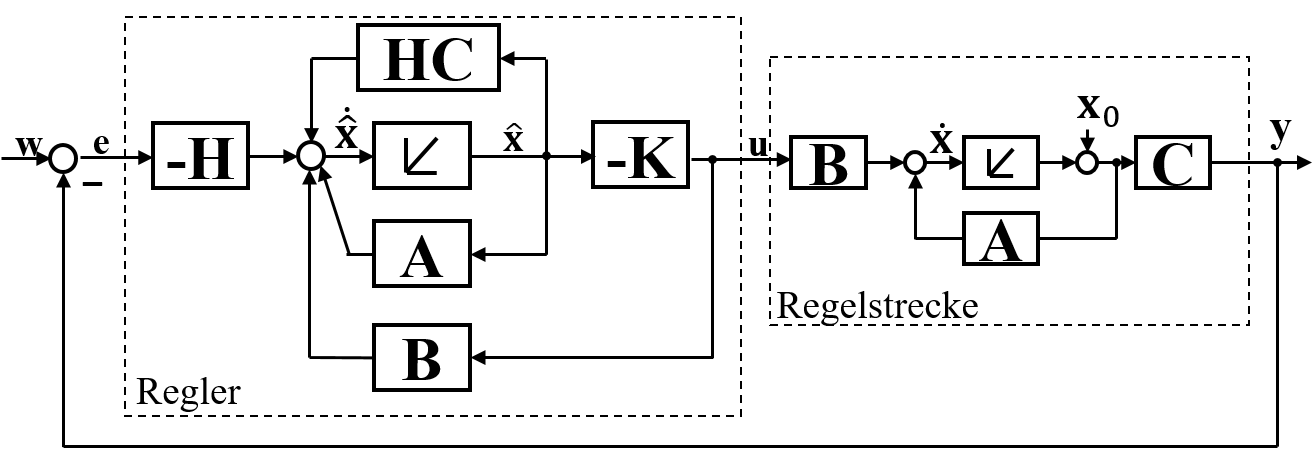
\includegraphics[width=0.4\linewidth]{bilder/observer_alternativ}
\end{center}
\begin{itemize}
	\item Dabei gelten die Gleichungen
	\item[] $\dot{\hat{x}} = \left( \boldsymbol{A}-\boldsymbol{BK}-\boldsymbol{HC}\right)\hat{x}-\boldsymbol{H}e$
	\item[] $u = -\boldsymbol{K}\hat{x}$
	\begin{itemize}
		\item Natürlich kann $e$ auch mit $w,\boldsymbol{A},\boldsymbol{B},\boldsymbol{C},\boldsymbol{K}$ ausgedrückt werden.
	\end{itemize}
	\item Für den Open-Loop ($w=0$) gilt:
	\item [] $G_o(s) = \boldsymbol{K}\left( s\boldsymbol{I}-\boldsymbol{A}+\boldsymbol{BK}+\boldsymbol{HC}\right)^{-1}\boldsymbol{H} \cdot\boldsymbol{C}\left(s\boldsymbol{I}-\boldsymbol{A}\right)^{-1}\boldsymbol{B}$
	\item Die Transferfuntktion des Reglers ist
	\item[] $G(s) = \frac{U(s)}{E(s)} = 
	\boldsymbol{K}\left( s\boldsymbol{I}-\boldsymbol{A}+\boldsymbol{BK}+\boldsymbol{HC}\right)^{-1}\boldsymbol{H}$
\end{itemize}

\subsection{LQG}
\begin{itemize}
	\item [1.] $\boldsymbol{AP}+\boldsymbol{PA}^T-\boldsymbol{PC}^T\boldsymbol{CP} ~~=-\rho\boldsymbol{BB}^T ~~=-\boldsymbol{Q}$
	\begin{itemize}
		\item Positiv definite Lösung von $\boldsymbol{P}$ wählen
	\end{itemize}
	\item [2.] $\boldsymbol{H} =\boldsymbol{PC}^T$
	\item Grosse Werte für $\rho ~~\Rightarrow$ Grosses Prozessrauschen führt zu grosser Verstärkung durch den Beobachter. Daher ist dieser anfälliger für verrauschte Signale.
\end{itemize}

\subsection{LTR (Loop transfer recovery)} 
\begin{itemize}
	\item LTR befasst sich mit der Platzierung der Pole von Regler und Beobachter, mit dem Ziel eine ausreichende Phasen- und Amplitudenreserve zu erreichen
	\item Die Phasen Reserve der einzelnen Teilsysteme ist min $\pm$\ang{60} und die Amplitudenreserve $\in \left[0.5\right. \ldots \infty \left.\right[$
	\item Das zusammengesetzte System hat jedoch \underline{keine} garantiert Reserve (weder Amplituden- noch Phasenreserve)
	\item Wird ein LQR (Regler) mit den Gewichtungsmatrizen ausgerechnet, erhalten wir die K-Matrix
	\item Wird ein LQG (Beobachter) mit den Gewichtungsmatrizen ausgerechnet, erhalten wir die H-Matrix
	\item Die H-Matrix wird entsprechnd der K-Matrix berechnet, wobei die Gewichtungen 
	\begin{itemize}
		\item $\boldsymbol{Q} = \rho \boldsymbol{BB}^T$ wobei $\boldsymbol{Q}$ das Prozessrauschen darstellt
		\item $\boldsymbol{R} = \boldsymbol{I}$ wobei $\boldsymbol{R}$ das Sensorrauschen darstellt
		\item Wenn R klein wird, wird Q gross und umgekehrt
	\end{itemize} 
	\item Bei einem minimalphasigen System gilt
	\item[] $\lim\limits_{\rho\rightarrow \infty}\left(G_o(s)\right) = \boldsymbol{K}\left(s\boldsymbol{I}-\boldsymbol{A}\right)^{-1}\boldsymbol{B}$
\end{itemize}

\subsubsection{Anwendung von LTR mit LQR und LQG}
\begin{itemize}
	\item Möglichkeit zum Erreichen der Reserve, wenn entweder der Regler oder der Beobachter beliebig gewichtet werden soll
\end{itemize}




\begin{tabularx}{\linewidth}{rp{.1\linewidth} rp{.1\linewidth}}
	\textbf{LQR beliebig}		&		&							\hspace{2.5cm} \textbf{LQG beliebig}& \\				
	Wert für LQR	&beliebig 										& 	Wert für LQR	&$\boldsymbol{Q} = \rho\boldsymbol{C}^T\boldsymbol{C}$\\
	Wert für LQG	&$\boldsymbol{Q} = \rho\boldsymbol{BB}$			& &	$\boldsymbol{R} = \boldsymbol{I}$ \\
					&$\boldsymbol{R} = \boldsymbol{I}$				& &	$\rho \ge 0$\\
					&$\rho \ge 0$									&Wert für LQG &beliebig	
\end{tabularx}
\newpage